
\begin{enumerate}

%%%%%%%%% Problem 1 %%%%%%%%%%%
    \item Create the DEPT table based on the following table instance chart. Place the
syntax in a script called \texttt{lab9\_1.sql}, then execute the statement in the script to create the table.
Confirm that the table is created
    \begin{figure}[h]
    \centering
        \centering
        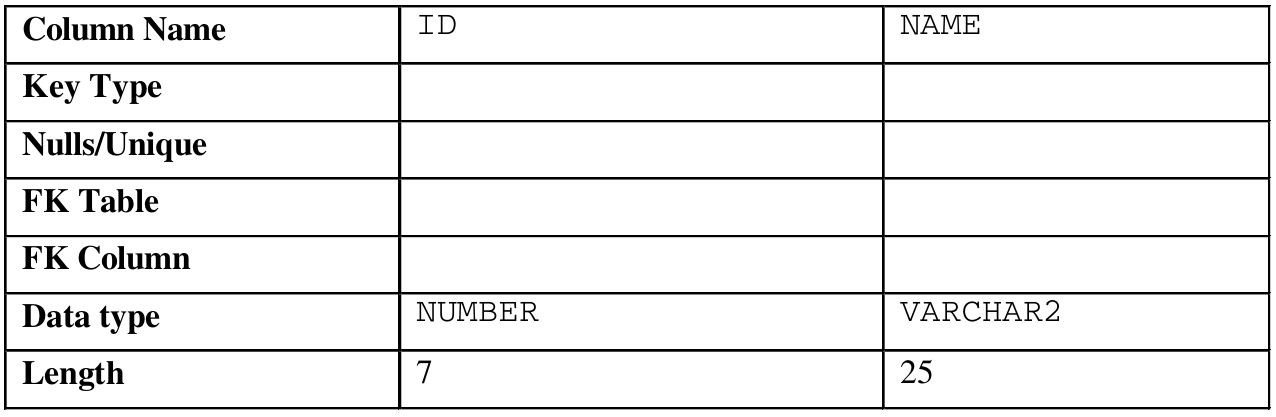
\includegraphics[width=.7\linewidth]{graphics/91.png}
    \end{figure}

    \textbf{Solution: }
    \begin{lstlisting}[language=SQL]
CREATE TABLE dept(
    ID INT (7),
    NAME VARCHAR(25)
);

DESCRIBE DEPT;
    \end{lstlisting}
    \textbf{Output: }
    \begin{figure}[h]
        \centering
        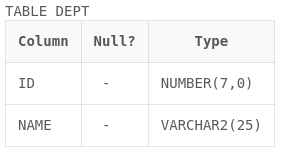
\includegraphics[width=0.5\linewidth]{graphics/p91.png}
    \end{figure}
%%%%%%%%% Problem 2 %%%%%%%%%%%
    \item Populate the DEPT table with data from the DEPARTMENTS table. Include only columns that
you need.

    \textbf{Solution: }
    \begin{lstlisting}[language=SQL]
INSERT INTO dept
SELECT department_id, department_name
FROM departments;
    \end{lstlisting}

%%%%%%%%% Problem 3 %%%%%%%%%%%
    \item Create the EMP table based on the following table instance chart. Place the syntax in a script called
\texttt{lab9\_3.sql}, and then execute the statement in the script to create the table. Confirm that the table is
created.
    \begin{figure}[h]
    \centering
        \centering
        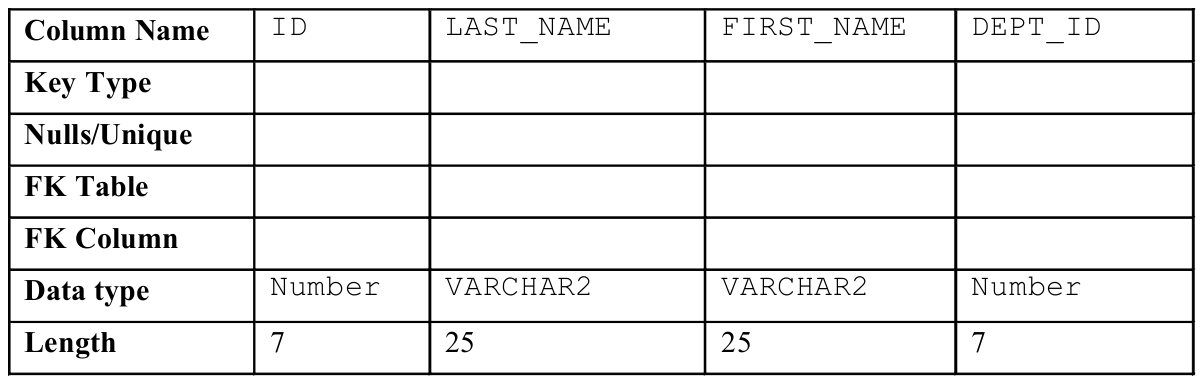
\includegraphics[width=.7\linewidth]{graphics/93.png}
    \end{figure}

    \textbf{Solution: }
    \begin{lstlisting}[language=SQL]
create table emp(
    id int (7),
    last_name varchar(25),
    first_name varchar(25),
    dept_id int (7)
);

DESCRIBE emp;
    \end{lstlisting}
    \textbf{Output: }
    \begin{figure}[h]
        \centering
        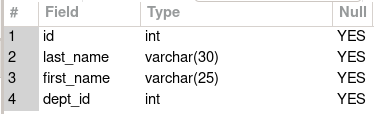
\includegraphics[width=0.5\linewidth]{graphics/p93.png}
    \end{figure}
%%%%%%%%% Problem 4 %%%%%%%%%%%
    \item Modify the EMP table to allow for longer employee last names. Confirm your modification.
    \begin{figure}[h]
    \centering
        \centering
        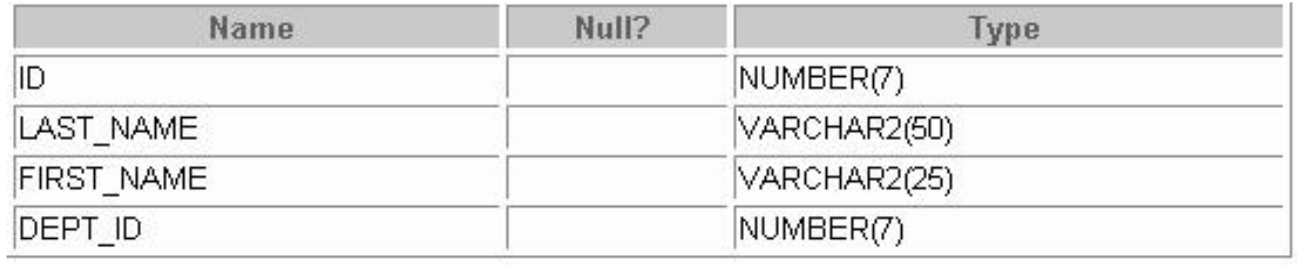
\includegraphics[width=.7\linewidth]{graphics/94.png}
    \end{figure}

    \textbf{Solution: }
    \begin{lstlisting}[language=SQL]
ALTER TABLE emp
MODIFY last_name VARCHAR(50);

DESCRIBE emp;
    \end{lstlisting}
    \textbf{Output: }
    \begin{figure}[h]
        \centering
        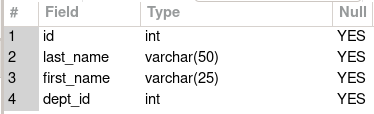
\includegraphics[width=0.5\linewidth]{graphics/p94.png}
    \end{figure}
%%%%%%%%% Problem 5 %%%%%%%%%%%

    \item Confirm that both the DEPT and EMP tables are stored in the data dictionary. (Hint:
\texttt{USER\_TABLES})
    \begin{figure}[h]
    \centering
        \centering
        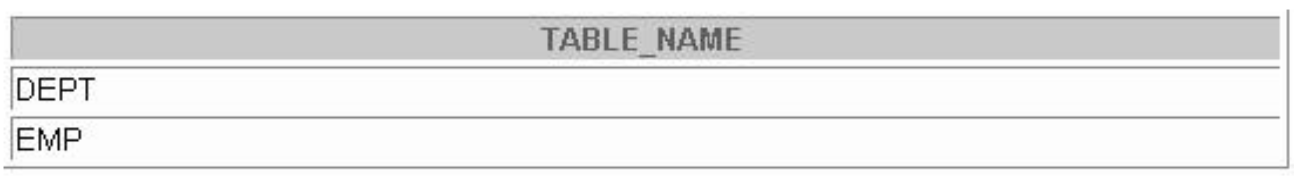
\includegraphics[width=.5\linewidth]{graphics/95.png}
    \end{figure}

    \textbf{Solution: }
    \begin{lstlisting}[language=SQL]
SELECT table_name
FROM information_schema.tables
WHERE table_name IN ('dept', 'emp');
    \end{lstlisting}
\textbf{Output: }
    \begin{figure}[h]
        \centering
        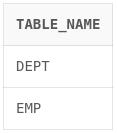
\includegraphics[width=0.5\linewidth]{graphics/p95.png}
    \end{figure}
%%%%%%%%% Problem 6 %%%%%%%%%%%
    \item \texttt{Create the EMPLOYEES2 table based on the structure of the EMPLOYEES table. Include only the
EMPLOYEE\_ID, FIRST\_NAME, LAST\_NAME, SALARY, and DEPARTMENT\_ID columns. Name
the columns in your new table ID, FIRST\_NAME, LAST\_NAME, SALARY , and DEPT\_ID,
respectively.}
    \begin{figure}[h]
    \centering
        \centering
        % 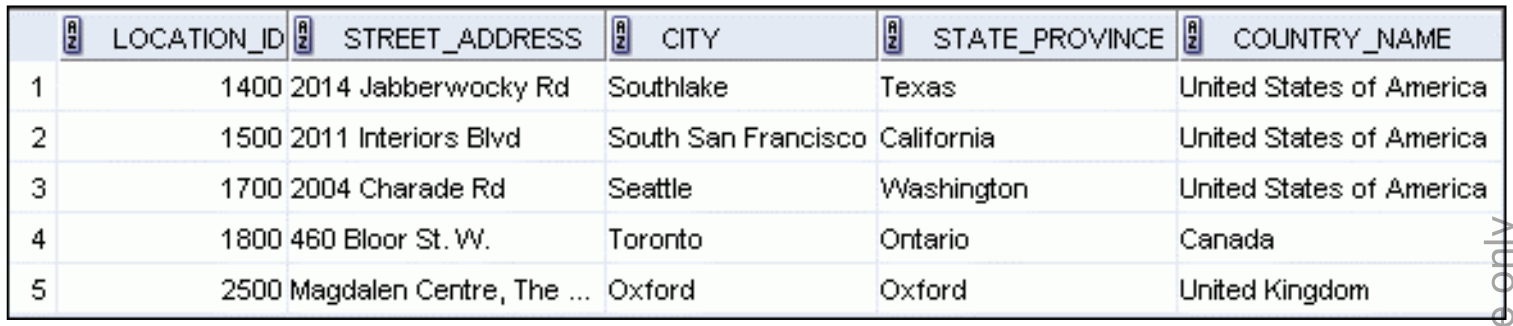
\includegraphics[width=.7\linewidth]{graphics/61.png}
    \end{figure}

    \textbf{Solution: }
    \begin{lstlisting}[language=SQL]
CREATE TABLE employees2 AS
SELECT employee_id id, first_name, last_name, salary,
    department_id dept_id
from employees;
    \end{lstlisting}

%%%%%%%%% Problem 7 %%%%%%%%%%%
    \item Drop the EMP table.
    \begin{figure}[h]
    \centering
        \centering
        % 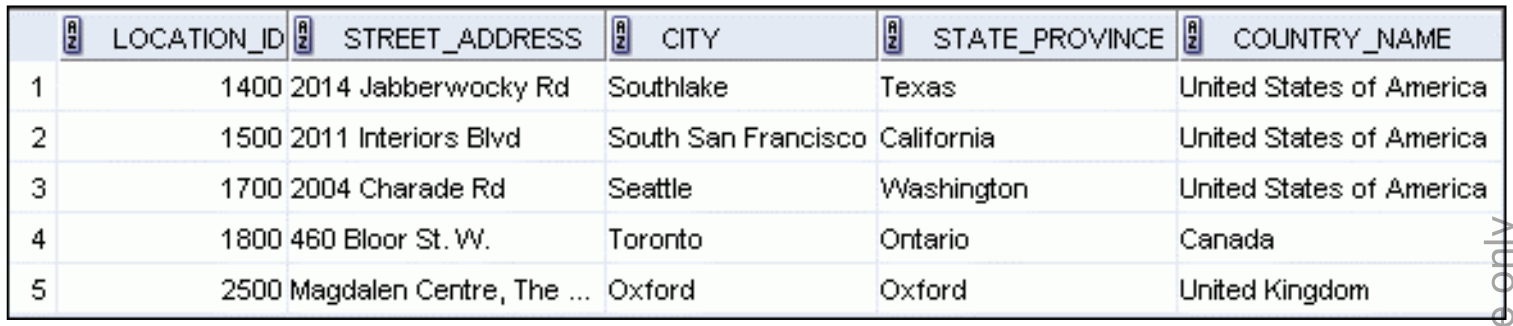
\includegraphics[width=.7\linewidth]{graphics/61.png}
    \end{figure}

    \textbf{Solution: }
    \begin{lstlisting}[language=SQL]
Drop table emp;
    \end{lstlisting}

%%%%%%%%% Problem 8 %%%%%%%%%%%
    \item Rename the EMPLOYEES2 table as EMP.
    \begin{figure}[h]
    \centering
        \centering
        % 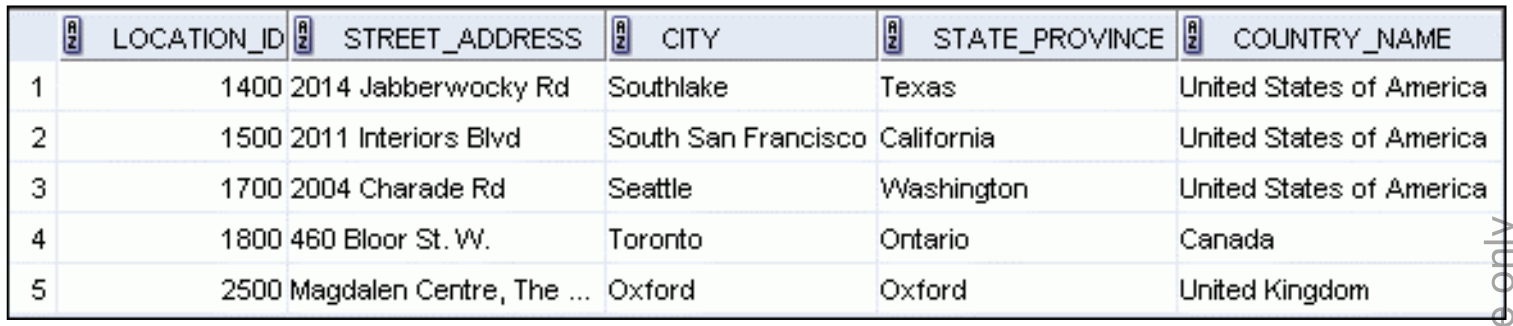
\includegraphics[width=.7\linewidth]{graphics/61.png}
    \end{figure}

    \textbf{Solution: }
    \begin{lstlisting}[language=SQL]
RENAME TABLE employees2 TO emp;
    \end{lstlisting}
\newpage
%%%%%%%%% Problem 9 %%%%%%%%%%%
    \item Add a comment to the DEPT and EMP table definitions describing the tables. Confirm your
additions in the data dictionary.

\textbf{Solution: }
    \begin{lstlisting}[language=SQL]
ALTER TABLE dept
COMMENT = 'This table stores department information';

ALTER TABLE emp
COMMENT = 'This table stores employee information';

SELECT table_name, table_comment
FROM information_schema.tables
WHERE table_name IN ('dept', 'emp');
    \end{lstlisting}
\textbf{Output: }
    \begin{figure}[h]
        \centering
        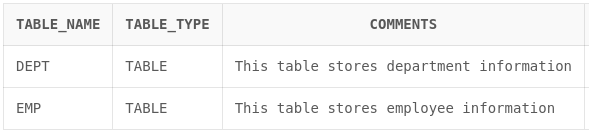
\includegraphics[width=0.8\linewidth]{graphics/p99.png}
    \end{figure}
    \newpage
%%%%%%%%% Problem 10 %%%%%%%%%%%
    \item Drop the \texttt{FIRST\_NAME} column from the EMP table. Confirm your modification by checking the
description of the table.

    \textbf{Solution: }
    \begin{lstlisting}[language=SQL]
alter table emp
drop last_name;

describe emp;
    \end{lstlisting}
    \textbf{Output: }
    \begin{figure}[h]
        \centering
        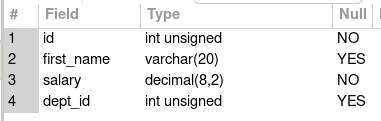
\includegraphics[width=0.5\linewidth]{graphics/p910.png}
    \end{figure}
%%%%%%%%% Problem 11 %%%%%%%%%%%
    \item In the EMP table, mark the \texttt{DEPT\_ID} column in the EMP table as UNUSED. Confirm your
modification by checking the description of the table.

    \textbf{Solution: }
    \begin{lstlisting}[language=SQL]
    \end{lstlisting}

%%%%%%%%% Problem 12 %%%%%%%%%%%
    \item In the EMP table, mark the \texttt{DEPT\_ID} column in the EMP table as UNUSED. Confirm your
modification by checking the description of the table.

    \textbf{Solution: }
    \begin{lstlisting}[language=SQL]
    \end{lstlisting}
\end{enumerate}